\section{実験\ref{sec:ex11}}
実験\ref{sec:ex1}の他のモデルにおける実験を行った。

\newpage
\subsection{モデル2の結果}
\begin{figure}[htbp]
    \begin{center}
        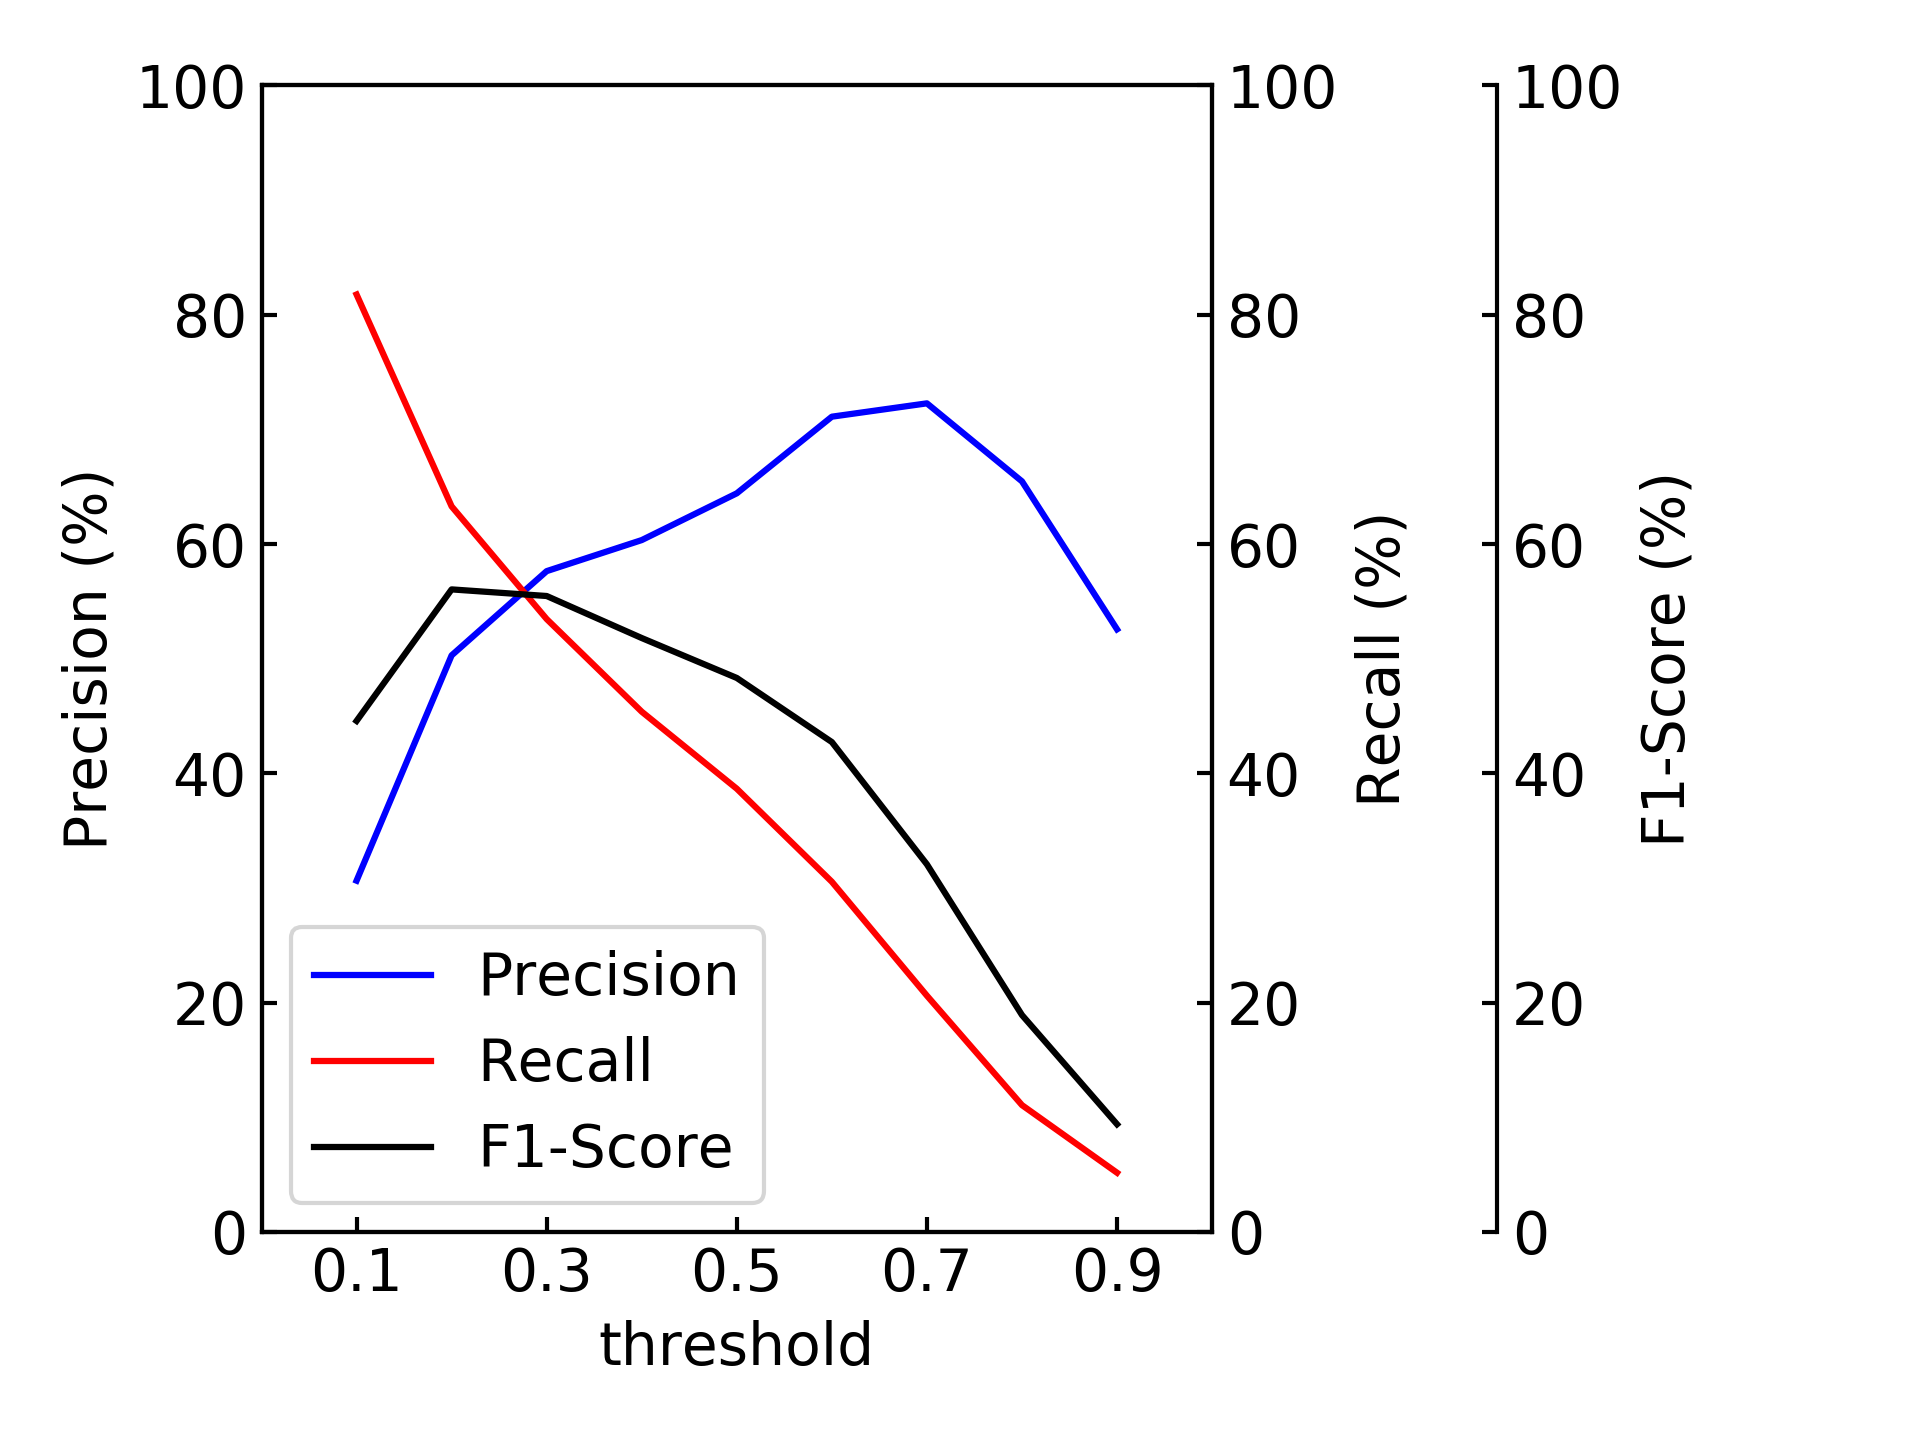
\includegraphics[width=150mm]{./fig/densenet121_e_p02threshold.png}
        \caption{しきい値を変化させた際の適合率と再現率の変化}
        \label{fig:densenet121_e_result_threshold}
    \end{center}
\end{figure}

\newpage
\subsection{モデル3の結果}
\begin{figure}[htbp]
    \begin{center}
        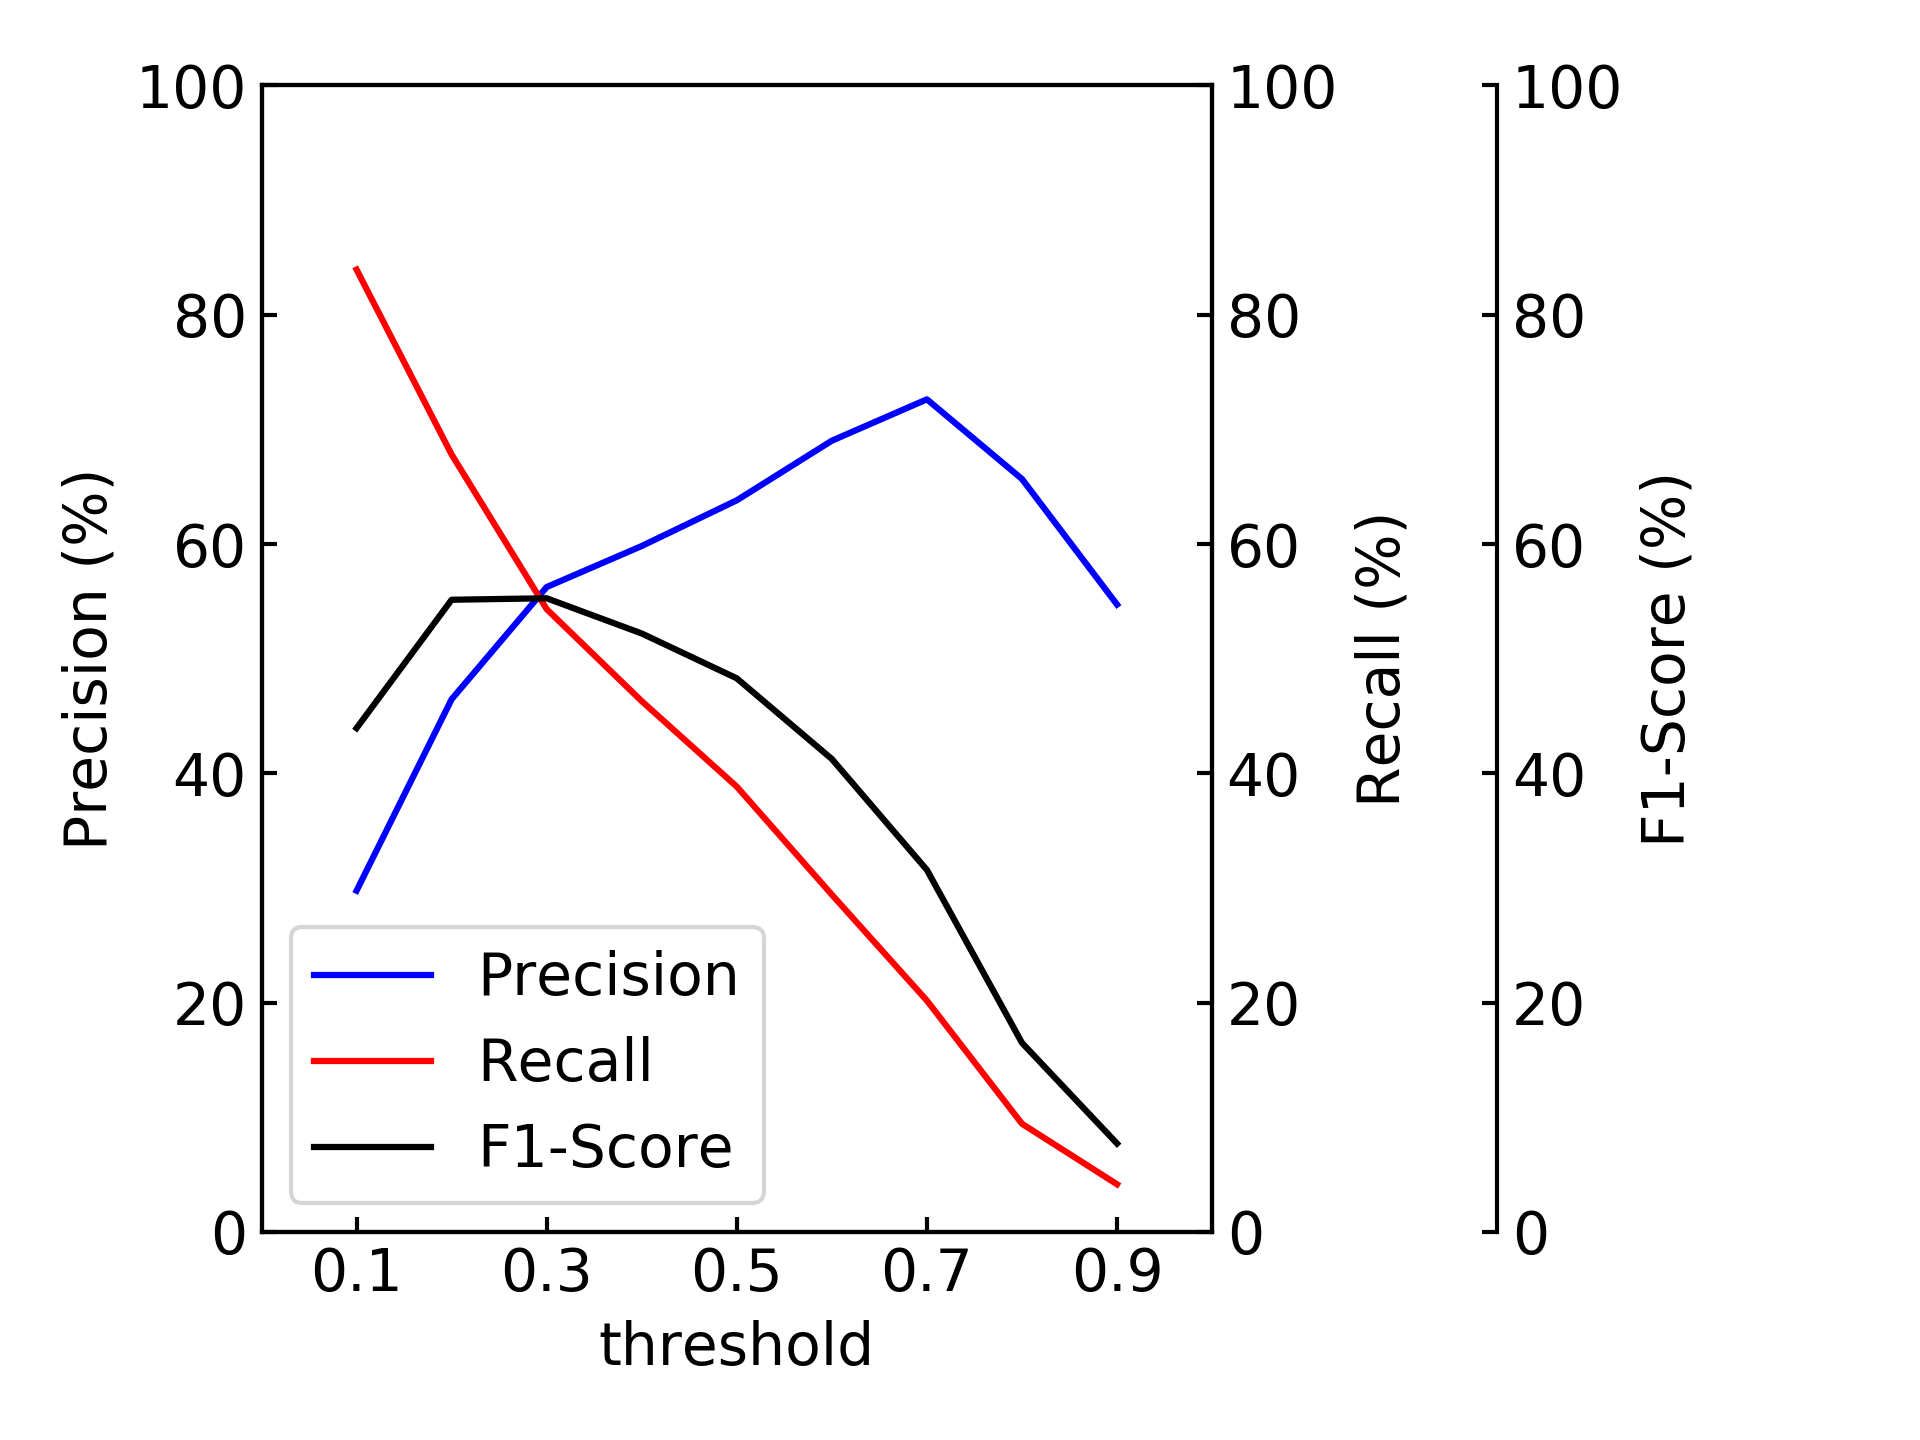
\includegraphics[width=150mm]{./fig/densenet161threshold.png}
        \caption{しきい値を変化させた際の適合率と再現率の変化}
        \label{fig:densenet161_result_threshold}
    \end{center}
\end{figure}

\newpage
\subsection{モデル4の結果}
\begin{figure}[htbp]
    \begin{center}
        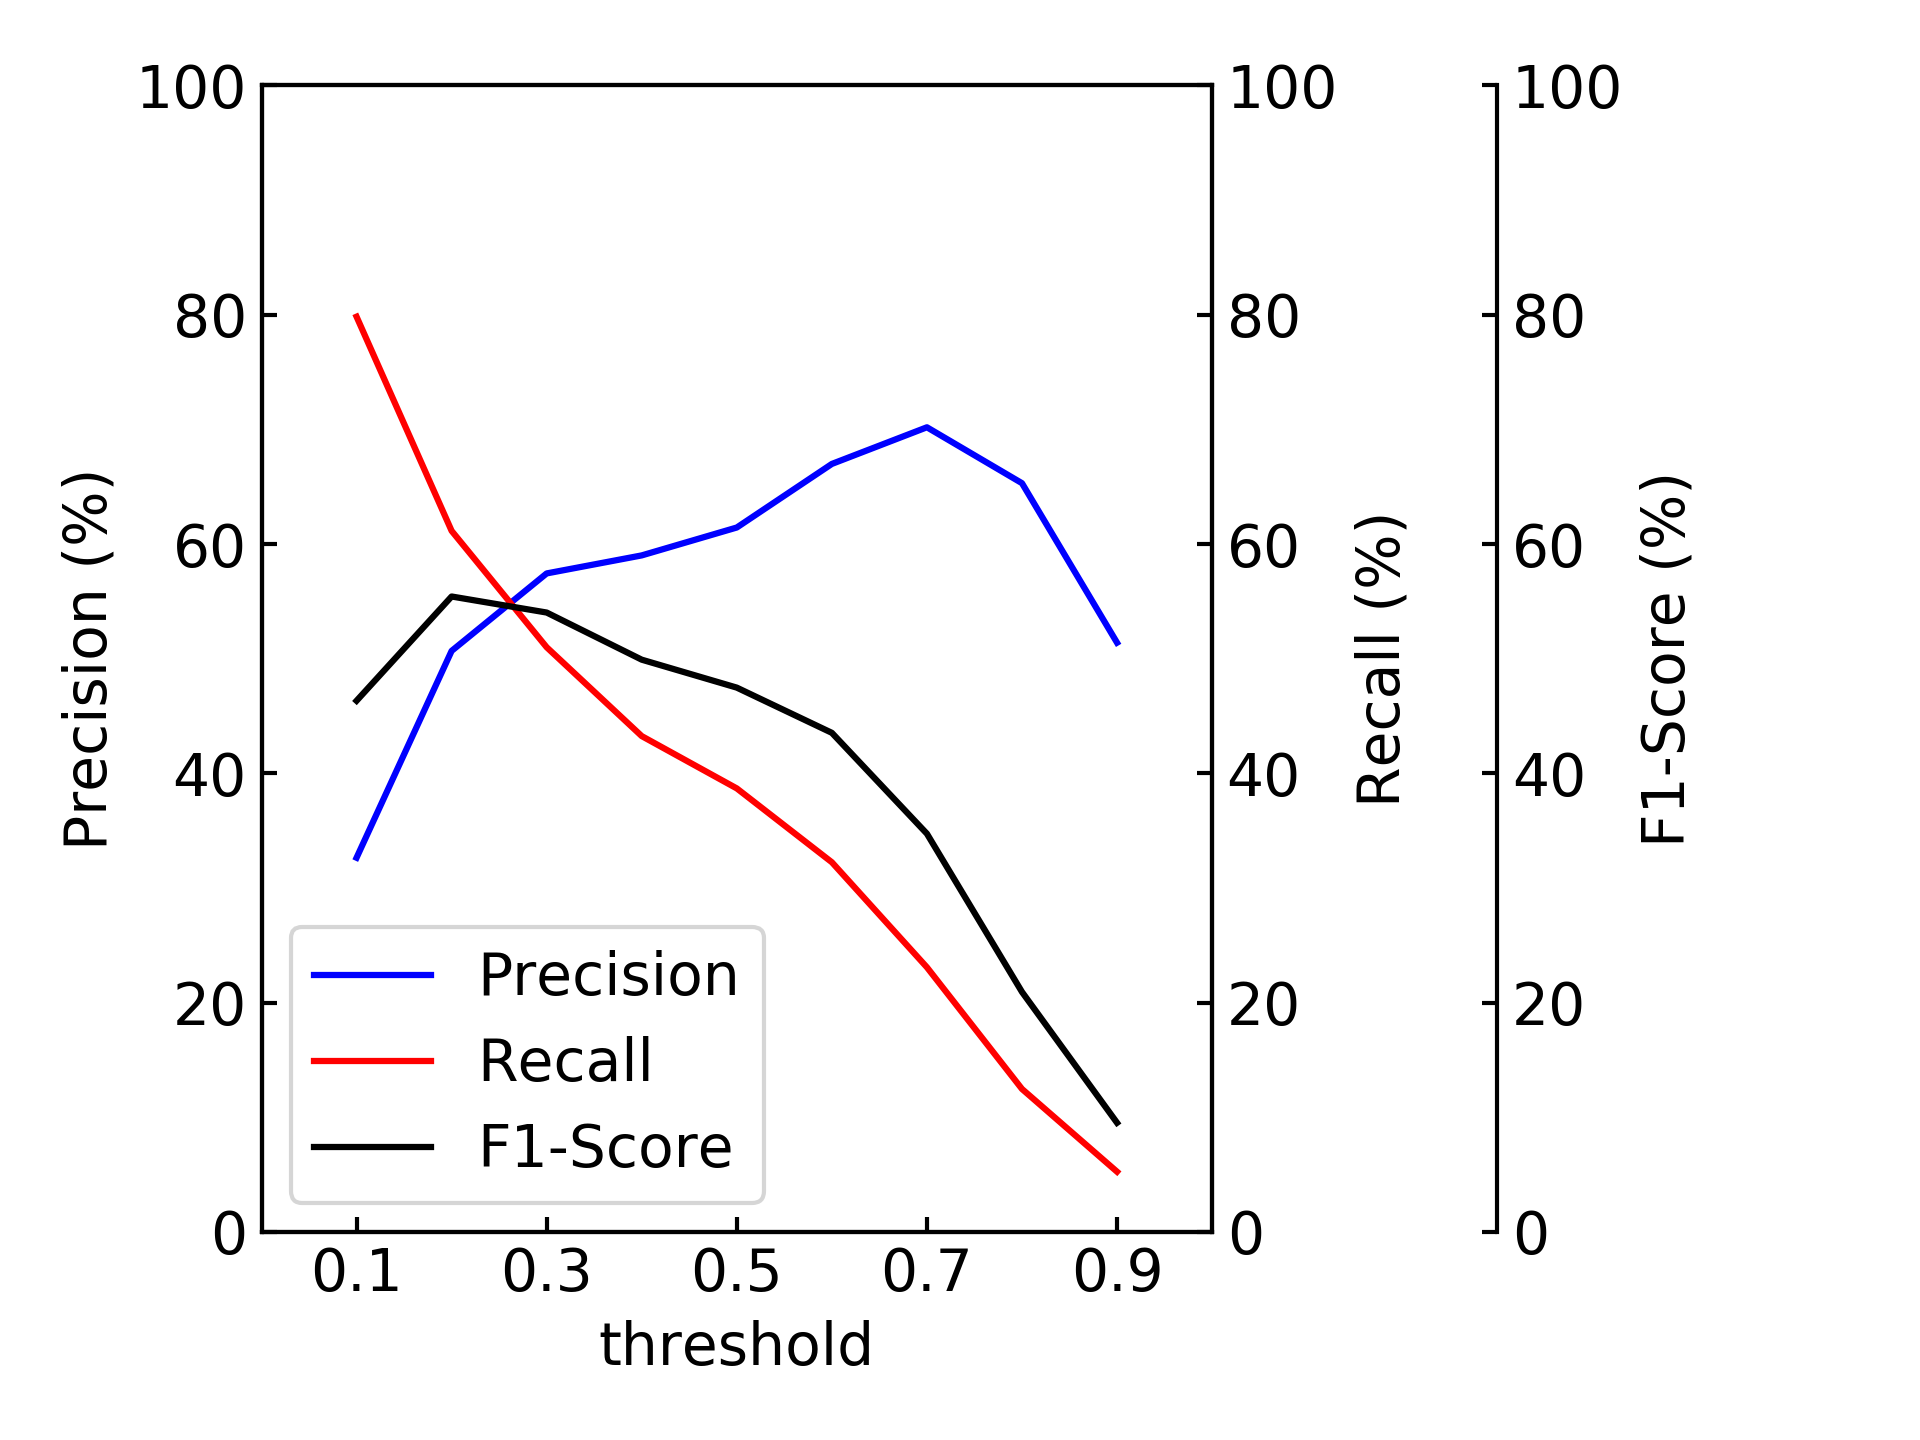
\includegraphics[width=150mm]{./fig/densenet161_ethreshold.png}
        \caption{しきい値を変化させた際の適合率と再現率の変化}
        \label{fig:densenet161_e_result_threshold}
    \end{center}
\end{figure}

\section{実験\ref{sec:ex22}}
実験\ref{sec:ex2}の他のモデルにおける実験を行った。

\newpage
\subsection{モデル2の結果}
\begin{figure}[htbp]
    \begin{center}
        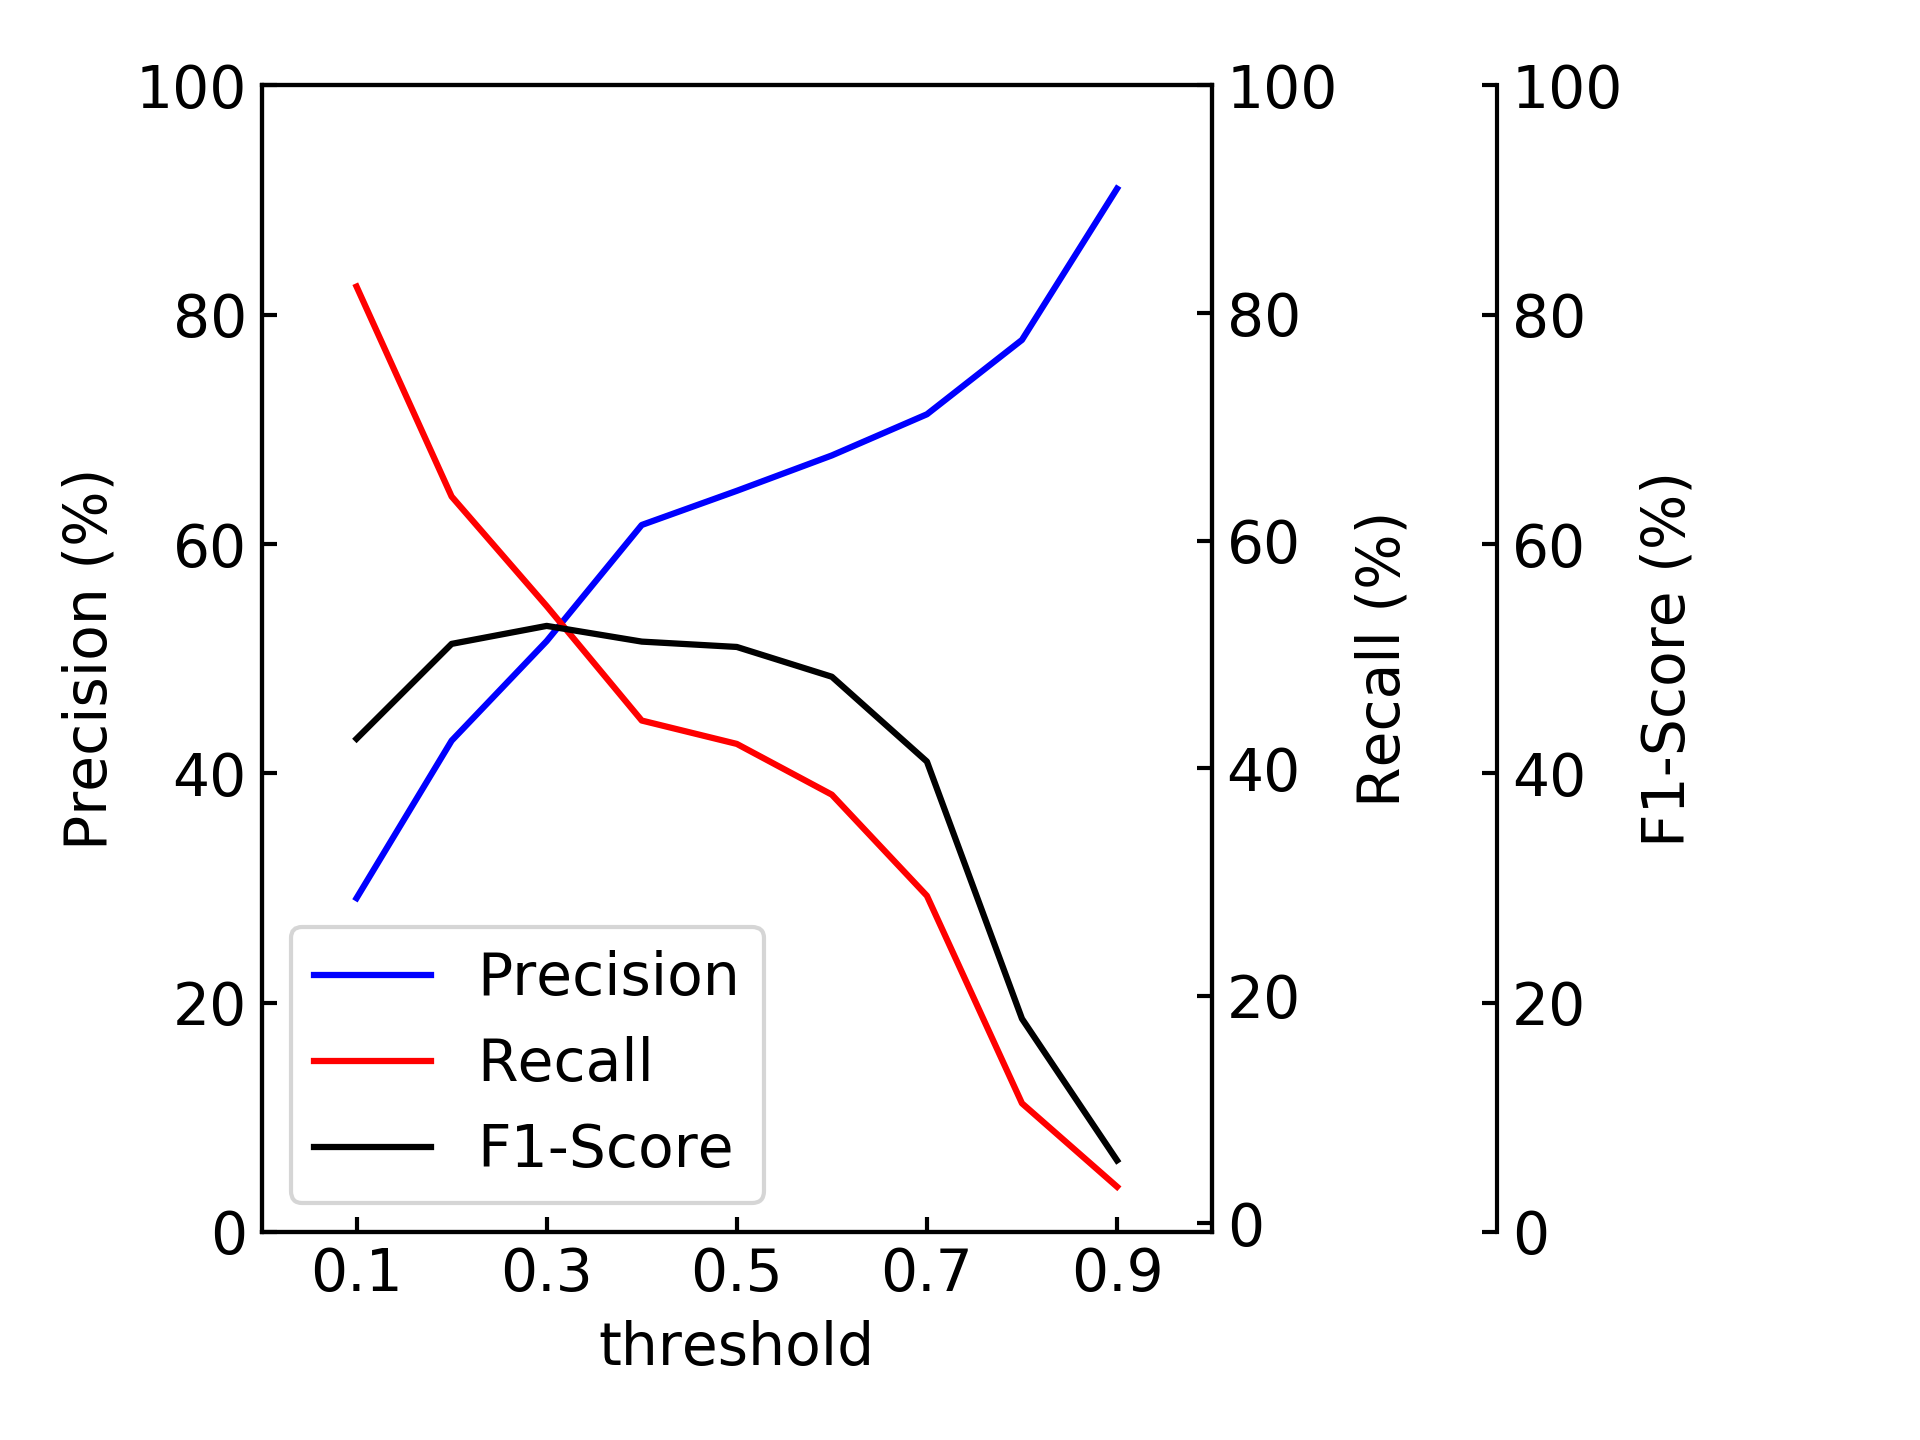
\includegraphics[width=150mm]{./fig/resnet3d_ethreshold.png}
        \caption{しきい値を変化させた際の適合率と再現率の変化}
        \label{figresnet3d_e_result_threshold}
    \end{center}
\end{figure}

\newpage
\subsection{モデル3の結果}
\begin{figure}[htbp]
    \begin{center}
        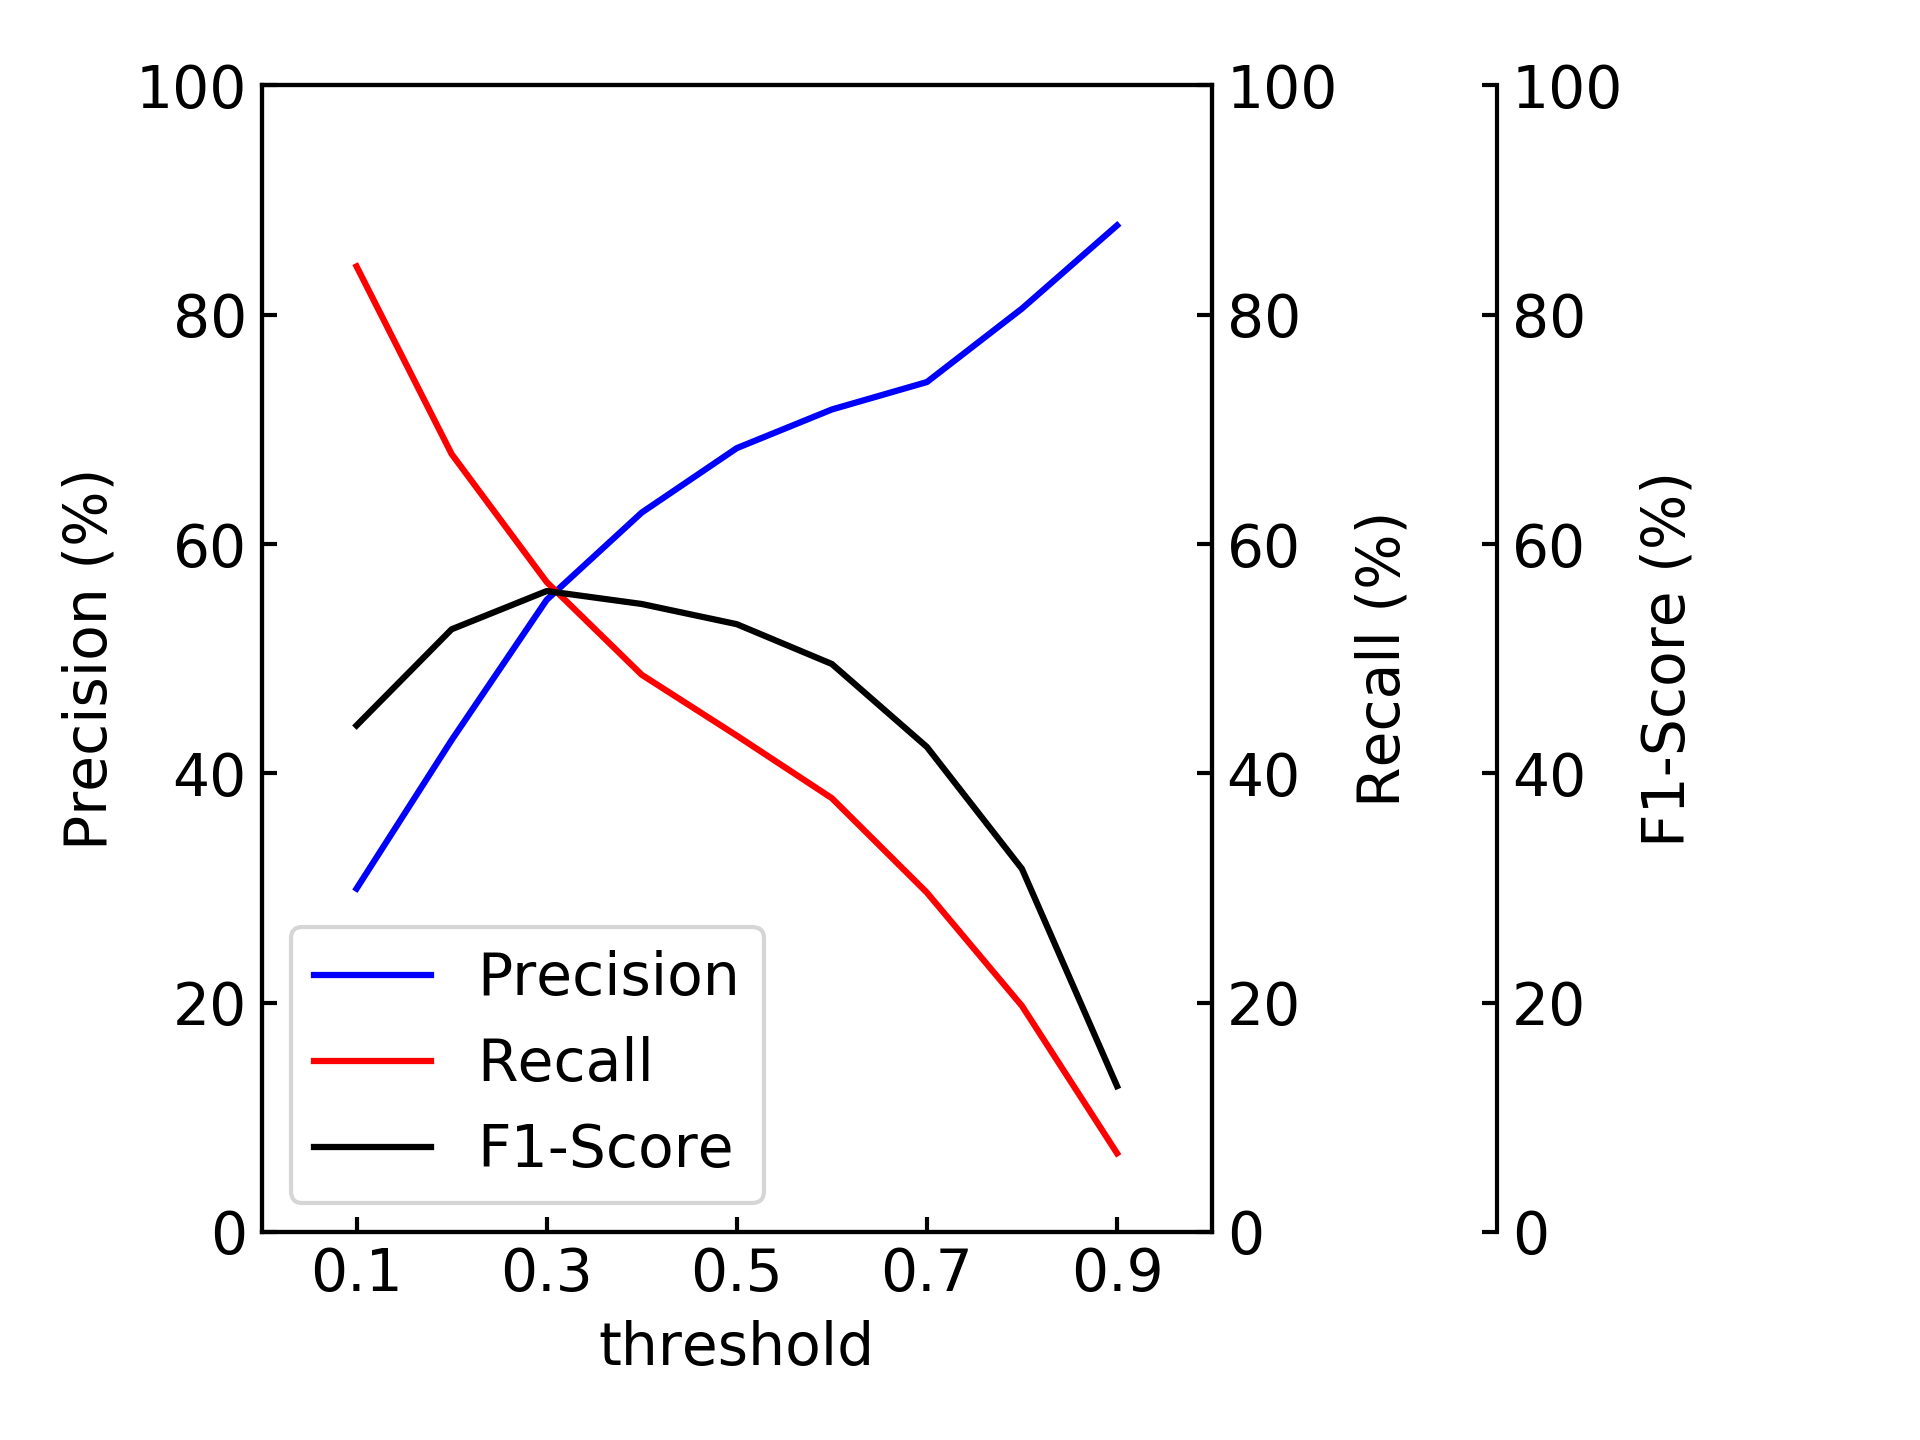
\includegraphics[width=150mm]{./fig/resnet3d_mthreshold.png}
        \caption{しきい値を変化させた際の適合率と再現率の変化}
        \label{fig:resnet3d_m_result_threshold}
    \end{center}
\end{figure}

\newpage
\subsection{モデル4の結果}
\begin{figure}[htbp]
    \begin{center}
        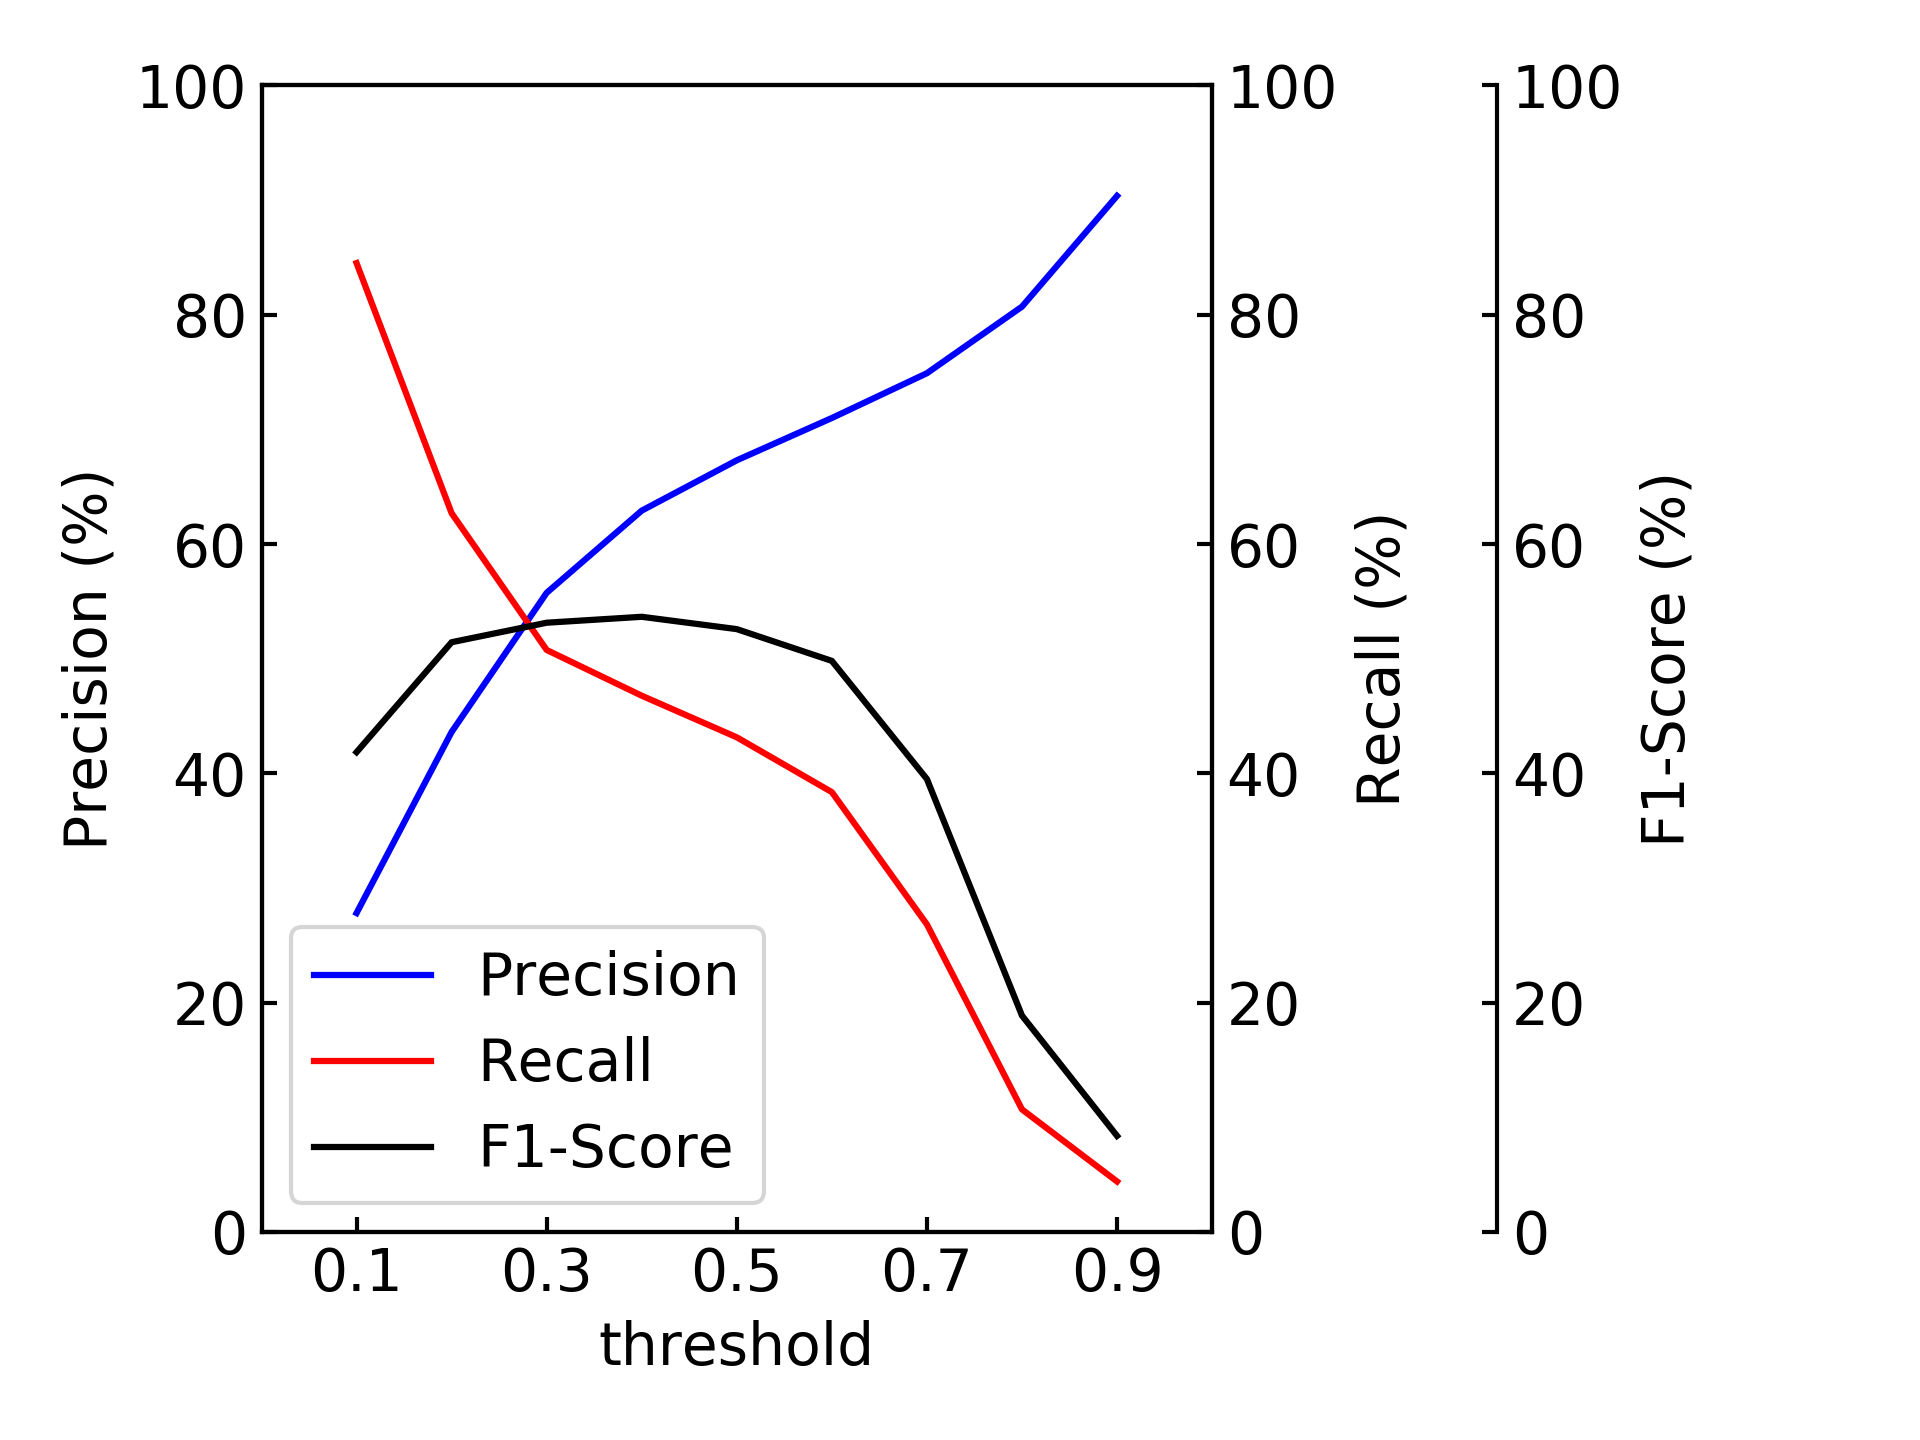
\includegraphics[width=150mm]{./fig/resnet3d_e_mthreshold.png}
        \caption{しきい値を変化させた際の適合率と再現率の変化}
        \label{fig:resnet3d_e_m_result_threshold}
    \end{center}
\end{figure}
